
\documentclass[a4paper,14pt, Times New Roman]{extarticle}
\linespread{1.1}
\usepackage[utf8]{inputenc}

\usepackage{geometry}

\usepackage[english, russian]{babel}

\usepackage{color}
\definecolor{bluekeywords}{rgb}{0.13,0.13,1}
\definecolor{greencomments}{rgb}{0,0.5,0}
\definecolor{redstrings}{rgb}{0.9,0,0}

\usepackage{listings}

\usepackage{graphicx}

\lstset{language=[Sharp]C,
extendedchars=\true,
inputencoding=utf8,
showspaces=false,
showtabs=false,
breaklines=true,
showstringspaces=false,
breakatwhitespace=true,
escapeinside={(*@}{@*)},
commentstyle=\color{greencomments},
keywordstyle=\color{bluekeywords}\bfseries,
stringstyle=\color{redstrings},
basicstyle=\ttfamily
}

\title{Отчёт по учебной практике}
\author{Грабовский Даниил Артемьевич}
\date{\today}

\graphicspath{ {RepotImages/} }

\begin{document}

\maketitle

\begin{center}
Тема: Кратчайшие пути на графе.
\end{center}

\begin{flushright}
Проверил преподаватель:

Теплоухов Семен Васильевич
\end{flushright}

\newpage

\renewcommand\contentsname{СОДЕРЖАНИЕ}

\tableofcontents

\newpage
\section{ВВЕДЕНИЕ}

Учебная практика является важным этапом в подготовки будущего специалиста. Непосредственное общение практиканта с новейшей вычислительной техникой, информационными и коммуникационными технологиями, приобретение им навыков работы в трудовом коллективе, участие в общественной жизни трудового коллектива – непременное условие формирования высококвалифицированного специалиста, члена информационного общества.

В настоящее время, в мире информационных технологий и компьютерной техники, одной из наиболее актуальных проблем является задача нахождения кратчайшего пути между двумя точками на карте. Это может быть необходимо, например, для оптимизации маршрутов в транспортных системах, планирования маршрутов доставки грузов, а также для решения других задач, связанных с навигацией и планированием.

Одним из наиболее эффективных алгоритмов для решения этой задачи является алгоритм Дейкстры, разработанный в 1959 году. Он позволяет находить кратчайшие пути между всеми парами вершин в графе, причем при этом не требуется знания о длине всех ребер графа.

Целью данной программы является реализация алгоритма Дейкстры на языке программирования C\# и его применение для нахождения кратчайших путей в графах, заданных в виде списков смежности. Программа позволяет пользователю задавать количество вершин в графе и определять начальную вершину. Результаты поиска кратчайшего пути выводятся на экран в виде списка ребер, которые образуют кратчайший путь между начальной вершиной и конечной вершиной. 
Алгоритм нахождения кратчайшего пути по критерию минимума затрат (алгоритм Дейкстры) может быть использован в различных областях, включая:

\begin{enumerate}
  \item Транспортную логистику - для нахождения кратчайшего маршрута между двумя точками с учетом стоимости проезда по каждому участку пути.
  \item Оптимизацию маршрутов доставки товаров - для определения наиболее эффективного маршрута доставки груза от производителя к конечному потребителю с учетом стоимости транспортировки и времени доставки.
  \item Маршрутизацию в сетях связи - для оптимизации маршрутизации трафика в сети с учетом затрат на передачу данных по каждому каналу связи.
  \item Оптимизацию работы систем управления - для определения наилучшего порядка выполнения задач с учетом времени выполнения и стоимости каждой задачи.
  \item Планировку маршрутов на местности - для поиска кратчайшего пути между двумя точками на карте с учетом рельефа местности и препятствий
\end{enumerate}

\newpage
\section{ОСНОВНАЯ ЧАСТЬ}

\subsection{Теоретическая часть}

\subsubsection{Алгоритм Дейкстры}

Алгоритм Дейкстры — алгоритм на графах, изобретённый нидерландским учёным Эдсгером Дейкстрой в 1959 году. Находит кратчайшие пути от одной из вершин графа до всех остальных. Алгоритм работает только для графов без рёбер отрицательного веса.

Известнo, что все цены неотрицательны. Найти наименьшую стоимость проезда 1->i для всех i=1..n за время O(n2).

В процессе работы алгоритма некоторые города будут выделенными (в начале - только город 1, в конце - все). При этом:

\begin{itemize}
  \item для каждого выделенного города i хранится наименьшая стоимость пути 1->i; при этом известно, что минимум достигается на пути, проходящем только через выделенные города;
  \item для каждого невыделенного города i хранится наименьшая стоимость пути 1->i, в котором в качестве промежуточных используются только выделенные города.
\end{itemize}

Множество выделенных городов расширяется на основании следующего замечания: если среди всех невыделенных городов взять тот, для которого хранимое число минимально, то это число является истинной наименьшей стоимостью. В самом деле, пусть есть более короткий путь. Рассмотрим первый невыделенный город на этом пути - уже до него путь длиннее! (Здесь существенна неотрицательность цен.)

Добавив выбранный город к выделенным, мы должны скорректировать информацию, хранимую для невыделенных городов. При этом достаточно учесть лишь пути, в которых новый город является последним пунктом пересадки, а это легко сделать, так как минимальную стоимость проезда в новый город мы уже знаем.

При самом бесхитростном способе хранения множества выделенных городов (в булевском векторе) добавление одного города к числу выделенных требует времени O(n).

Алгоритм использует три массива из N (= числу вершин сети) чисел каждый. Первый массив S содержит метки с двумя значения: 0 (вершина еще не рассмотрена) и 1 (вершина уже рассмотрена); второй массив B содержит расстояния - текущие кратчайшие рас- стояния от до соответствующей вершины; третий массив с содержит номера вершин - k-й элемент С[k] есть номер предпоследней вершины на текущем кратчайшем пути из Vi в Vk. Матрица расстояний A[i,k] задает длины дуге A[i,k]; если такой дуги нет, то A[i,k] присваивается большое число Б, равное "машинной бесконечности".

\subsubsection{Язык программирования C\#}

C\# (читается как си шарп) - это объектно-ориентированный язык программирования, разработанный компанией Microsoft в 2000 году. Он является частью платформы .NET Framework и используется для разработки приложений на Windows, Android, iOS и других платформах.

Синтаксис C\# похож на язык Java, но он более простой и понятный для начинающих программистов. C\# поддерживает различные типы данных, включая целочисленные, вещественные, строковые, логические и массивы. Также он имеет встроенные средства для работы с файлами, сетью, базами данных и другие.

C\# имеет объектно-ориентированную модель разработки, которая позволяет создавать классы и объекты, наследовать их, переопределять методы и свойства. Классы в C\# могут иметь атрибуты, события, индексаторы и делегаты.

Объектно-ориентированное программирование (ООП) - это методология программирования, которая основывается на концепции объектов. Объекты представляют собой экземпляры классов, которые определяют свойства и поведение этих объектов.

Основная идея ООП заключается в том, чтобы разделить программу на отдельные компоненты, называемые объектами, каждый из которых имеет свои собственные свойства и методы. Это позволяет создавать более модульный и гибкий код, который легче тестировать и поддерживать.

ООП имеет множество преимуществ, таких как упрощение структуры программы, повышение ее модульности и надежности, а также возможность повторного использования кода. Кроме того, ООП позволяет более эффективно использовать ресурсы компьютера, так как объекты могут быть созданы и уничтожены динамически, что уменьшает нагрузку на память.

Для написания кода на C\# можно использовать интегрированную среду разработки (IDE), такую как Visual Studio или MonoDevelop. IDE предоставляет множество инструментов для отладки, тестирования, сборки и развертывания приложений.
Преимущества языка программирования C\#:

\begin{enumerate}
  \item Простота и удобство использования: C\# является простым и удобным языком программирования, который позволяет разработчикам быстро создавать приложения и веб-сайты.
  \item Поддержка объектно-ориентированного программирования: C\# поддерживает объектно-ориентированное программирование, что позволяет создавать более гибкие и масштабируемые приложения.
  \item Широкие возможности для работы с базами данных: C\# имеет мощные средства для работы с различными базами данных, такими как SQL Server, MySQL и другие.
  \item Кроссплатформенность: C\# может использоваться для создания приложений для различных платформ, таких как Windows, Linux и macOS.
  \item Интеграция с другими языками программирования: C\# обладает возможностью интеграции с другими языками программирования, такими как Java и Python.
  \item Широкий спектр библиотек и инструментов: Существует множество библиотек и инструментов для работы с C\#, которые облегчают разработку приложений.
  \item Доступность и поддержка: C\# широко используется в индустрии разработки программного обеспечения и имеет хорошую поддержку сообщества разработчиков.
\end{enumerate}

\subsubsection{Платформа .NET Framework}

Microsoft .NET Framework - это программная платформа, которая обеспечивает основу для разработки и исполнения приложений на языке C или Visual Basic.NET, а также других языков .NET.

Основные функции, которые предоставляет .NET Framework, включают:


\begin{itemize}
  \item Безопасность: .NET Framework обеспечивает безопасность приложений, предоставляя механизмы защиты от атак, таких как SQL-инъекции и XSS.
  \item Управление памятью: .NET Framework предоставляет механизмы управления памятью, такие как сборщик мусора, что позволяет приложениям работать более эффективно.
  \item Обработка исключений: .NET Framework позволяет приложениям обрабатывать исключения, что делает их более устойчивыми к ошибкам.
  \item Работа с файлами и сетью: .NET Framework предоставляет API для работы с файлами, сетью и другими ресурсами.
  \item Поддержка многопоточности: .NET Framework поддерживает многопоточность, что позволяет разрабатывать приложения, которые могут обрабатывать несколько задач одновременно.
\end{itemize}

Вот некоторые из преимуществ платформы Net Framework:

\begin{enumerate}
  \item Кроссплатформенность: Благодаря использованию Net Framework, приложения могут работать на различных версиях Windows, что обеспечивает их совместимость и кроссплатформенность.
  \item Безопасность: Net Framework предоставляет более безопасные API для работы с файлами, сетью и другими ресурсами, что повышает уровень безопасности приложений.
  \item Масштабируемость: Net Framework поддерживает масштабируемость приложений, позволяя добавлять новые функции и компоненты без необходимости переписывать весь код.
  \item Удобство использования: Платформа Net Framework обеспечивает простой и удобный способ создания приложений для Windows, предоставляя готовые инструменты и библиотеки для работы с различными компонентами.
  \item Поддержка сообщества: Платформа Net Framework имеет активное сообщество разработчиков, которое поддерживает и обновляет ее, обеспечивая стабильность и безопасность.
\end{enumerate}

\subsubsection{Библиотека Windows Forms}

Библиотека для создания приложений с графическим интерфейсом Windows Forms - это набор инструментов и компонентов, которые позволяют разработчикам создавать пользовательские интерфейсы для своих приложений на платформе Windows. Она включает в себя такие компоненты, как кнопки, текстовые поля, списки, таблицы, флажки, радиокнопки, ползунки и другие элементы управления, которые можно использовать для создания пользовательских интерфейсов.

Библиотека Windows Forms предоставляет разработчикам удобный способ создания графических интерфейсов для приложений. Она позволяет создавать приложения, которые могут быть легко настроены и модифицированы в соответствии с потребностями пользователя. Библиотека также позволяет создавать программы, которые могут работать на разных версиях операционной системы Windows, что делает ее широко используемой.

Преимущества Windows Forms:

\begin{enumerate}
  \item Простота использования: Windows Forms предоставляет интуитивно понятный интерфейс для создания пользовательского интерфейса приложения.
  \item Гибкость: Windows Forms позволяет создавать приложения с различными стилями и функциональностью, в зависимости от требований пользователя.
  \item Надежность: Windows Forms имеет широкий спектр библиотек и компонентов, которые обеспечивают стабильность и надежность приложения.
  \item Поддержка: Microsoft предоставляет обширную документацию и поддержку сообщества разработчиков, что упрощает разработку приложений на основе Windows Forms.
  \item Кроссплатформенность: Приложения, созданные на основе Windows Forms, могут работать на различных платформах, таких как Windows, macOS и Linux.
\end{enumerate}

\subsection{Практическая часть}

\subsubsection{Постановка задачи}
Разработать программу, которая будет использовать алгоритм Дейкстры для нахождения кратчайшего пути от заданной начальной точки до всех остальных точек на заданном графе. Граф может быть представлен в виде матрицы смежности или списка смежности. Программа должна поддерживать возможность изменения начальной точки и проверку корректности графа

\subsubsection{Разработка класса Vector}
Класс - это шаблон для создания объектов, которые могут быть использованы для выполнения определенных задач. Класс определяет свойства и методы, которые доступны для объектов этого класса.

Объект - это экземпляр класса, который создается при его создании. Объекты имеют свои собственные значения свойств и могут вызывать методы класса. Они также могут быть переданы в качестве параметров в методы других классов.

Метод - это блок кода, который может быть вызван из другого места программы. Метод возвращает значение типа, указанного в его определении.

Методы в C могут быть определены внутри классов, структур и интерфейсов. Методы могут иметь параметры, которые передаются им при вызове.

Поле - это переменная, которая находится внутри класса и может использоваться только внутри этого класса. Поля могут быть объявлены как общедоступные, защищенные или частные.

Классы и объекты являются фундаментальными понятиями в объектно-ориентированном программировании и используются для создания программ, которые работают с данными и выполняют задачи.

Для разработки программы поиска короткого пути в графе, я решил разработать класс Vector и Relation.

Класс Vector будет хранить информацию о координатах (X,Y), названии точки (Name), размер точки (Size) и состояния фокуса (Focused) и выделения точки (Selected).

\begin{lstlisting}
public float X;
public float Y;
public float Size;
public string Name;
public bool Selected;
public bool Focused
\end{lstlisting}

Конструктор класса Vector будет подготавливать значение некоторых переменных(полей) класса.

\begin{lstlisting}
public Vector(float x, float y, string name)
{
    X = x;
    Y = y;
    Name = name;
    Size = 4;
}
\end{lstlisting}

Для определения угла между двумя точками (Vector) на плоскости была создана функции (метод) GetAngle, в параметры которой будет указываться вторая точка (Vector), координаты первой точки прописаны в самом классе.

\begin{lstlisting}
public double GetAngle(Vector b)
{
    return Math.Atan2(b.Y, b.X) - Math.Atan2(this.Y, this.X);
}
\end{lstlisting}

Функция GetDistance по теореме Пифагора определяет расстояние между двумя точками. В качестве параметра указывается вторая точка, координаты первой точки прописаны в самом классе.

\begin{lstlisting}
public double GetDistance(Vector b)
{
    double _x = Math.Abs(X - b.X);
    double _y = Math.Abs(Y - b.Y);
    return Math.Sqrt(Math.Abs(_x * _x - _y * _y));
}
\end{lstlisting}

\subsubsection{Разработка класса Relation}

Класс  Relation описывает взаимодействие двух Vector, направление стрелки (Reverse) или двух стороннее направление (Duplex), и состояние выделения Relation.

\begin{lstlisting}
public Vector VectorA;
public Vector VectorB;
public bool Reverse = false;
public bool Duplex = false;
public bool Selected = false;
\end{lstlisting}

В конструкторе класса Relation в качестве параметров указываются две точки(Vector), между которыми необходимо установить связь(Relation), направление стрелки с помощью параметра reverse, и  двухстороннюю связь duplex.

\begin{lstlisting}
public Relation(Vector vectorA, Vector vectorB, bool reverse, bool duplex)
{
    this.vectorA = vectorA;
    this.vectorB = vectorB;
    this.Reverse = reverse;
    this.Duplex = duplex;
}
\end{lstlisting}

Функция GetAngle в Relation определяет угол между двумя точками.

\begin{lstlisting}
public double GetAngle()
{
    if (VectorA != VectorB)
    {
        if ((VectorA != null) && (VectorB != null))
        {
            double angle = Math.Atan2(VectorB.Y, VectorB.X) - Math.Atan2(VectorA.Y, VectorA.X);
            return angle;
        }
    }
    return 0;
}
\end{lstlisting}

Функция Distance в Relation определяет расстояние между двумя точками.

\begin{lstlisting}
public double Distance(int dec = 1)
{
    double x = Math.Abs(VectorA.X - VectorB.X);
    double y = Math.Abs(VectorA.Y - VectorB.Y);
    double d = Math.Sqrt(x * x + y * y);
    return Math.Round(d, dec);
}
\end{lstlisting}

Функция Select в Relation задаёт состояние выделения двух точек.

\begin{lstlisting}
public void Select(bool value = true)
{
    Selected = value;
    vectorA.Selected = value;
    vectorB.Selected = value;
}
\end{lstlisting}

\subsubsection{Разработка компонента управления}

После разработки двух классов, я решил разработать главный класс, в котором будет выполняться решение задачи.

Для хранения точек на плоскости я использовал словарь Vectors. 

Словарь - это структура данных, которая позволяет хранить пары ключ-значение. В C словарь реализуется через класс Dictionary. Словарь в C\# может быть реализован как хэш-таблица или как дерево.

Словари в языке C\# предоставляют множество преимуществ, которые делают их очень полезными при разработке программ. Некоторые из основных преимуществ словарей в C\# включают:

\begin{enumerate}
  \item Легкость использования: Словари очень легко использовать, так как они предоставляют простой интерфейс для добавления, удаления и получения элементов.
  \item Эффективность: Словари могут быть очень эффективными при работе с большими объемами данных, так как они используют хэш-таблицы для быстрого доступа к элементам.
  \item Поддержка множественного значения: Словари позволяют хранить элементы с множественным значением, что делает их удобными для работы с данными, которые могут иметь несколько значений для одного ключа.
  \item Удобство использования: Словари предоставляют удобный способ организации данных в виде ассоциативного массива, что позволяет легко обращаться к элементам по ключу.
  \item Безопасность: Словари обеспечивают безопасность данных, так как ключи и значения хранятся в зашифрованном виде и доступ к ним ограничен.
\end{enumerate}

В словаре Vectors в качестве ключа указывается уникальное имя точки, что бы в программе можно было по ней обратиться, качестве значения указывается объект класса Vector.

Для описания связей (Relations) использовались списки.

Списки (List) - это один из основных типов данных в языке программирования C\#. Списки позволяют хранить и обрабатывать коллекции элементов одного типа.

Списки в C могут использоваться для хранения и обработки информации, например, для хранения списка пользователей в базе данных или для хранения элементов в списке товаров. Они также могут использоваться для создания алгоритмов и структур данных, таких как стеки и очереди.

В списке Relations хранится список связей между точками.

\begin{lstlisting}
Dictionary<object, Vector> Vectors;
List<Relation> Relations;
\end{lstlisting}

Функция GetPoints получает в данные обо всех точках в виде массива.

\begin{lstlisting}
public object[] GetPoints()
{
    return Vectors.Keys.ToArray();
}
\end{lstlisting}

В методе InitializeVariables подготавливаются переменные Vectors и Relations.

\begin{lstlisting}
private void InitializeVariables()
{
Vectors = new Dictionary<object, Vector>();
Relations = new List<Relation>();
}
\end{lstlisting}

Метод AddPoint добавляет точку в словарь Vectors. В качестве параметра указывается символ точки, позиция по оси X, позиция по оси Y, и имя точки.

\begin{lstlisting}
public void AddPoint(char point, int x, int y, string name = "")
{
    Vectors.Add(point, Vector.Create(x, y, name));
}
\end{lstlisting}

Метод AddRelation добавляет связь двумя точками в список Relations. В качестве параметра указывается символы двух точек, направление стрелки reverse, и двухстороннюю связь duplex. Указания символов точек необходимо для того, что бы метод выбирал значения только из словаря, тем самым предотвращая добавление на точки Vector, не существующей на плоскости.

\begin{lstlisting}
public void AddRelation(char pointA, char pointB, bool reverse = false, bool duplex = false)
{
    Vector a;
    Vector b;
    Vectors.TryGetValue(pointA, out a);
    Vectors.TryGetValue(pointB, out b);
    Relations.Add(Relation.Create(a, b, reverse, duplex));
}
\end{lstlisting}

Метод GetRelations получает список всех Связей(Relation), которые связаны с конкретной точкой (Vector). Путём перебора общего списка связей Relations, выбираются только те, которые равны с заданной точкой

\begin{lstlisting}
private List<Relation> GetRelations(Vector vector)
{
    List<Relation> relations = new List<Relation>();
    if (vector != null)
    {
        foreach (Relation relation in Relations)
        {
            if (relation != null)
                if (relation.VectorA == vector)
                    relations.Add(relation);
        }
    }
    return relations;
}
\end{lstlisting}

Метод GetRelation получает только одну связь, которая была найдена из общего списка по двум точкам (Vector)

\begin{lstlisting}
private Relation GetRelation(Vector vectorA, Vector vectorB)
{
    if (vectorA != null && vectorB != null)
    {
        foreach (Relation relation in Relations)
        {
            if (relation != null)
            {
                if (relation.Duplex)
                {
                    if (relation.VectorA == vectorA && relation.VectorB == vectorB ||
                        relation.VectorA == vectorB && relation.VectorB == vectorA)
                    return relation;
                }
                else if (!relation.Reverse)
                {
                    if (relation.VectorA == vectorA && relation.VectorB == vectorB)
                    return relation;
                }
                else
                {
                    if (relation.VectorA == vectorB && relation.VectorB == vectorA)
                        return relation;
                }
            }
        }
    }
    return null;
}
\end{lstlisting}

Метод HasRelation проверяет существование связи для указанной в параметрах точки.

\begin{lstlisting}
private bool HasRelation(Vector vector)
{
    if (vector != null)
    {
        foreach (Relation relation in Relations)
        {
            if (relation != null)
                if (relation.VectorA == vector || relation.VectorB == vector)
                    return true;
        }
    }
    return false;
}
\end{lstlisting}

\subsubsection{Разработка управляющих функций}
После разработки функций для управления, были разработаны функции, которые участвую уже непосредственно в решении задачи. 

Матрица путей WaysDistance находится стоимости пути, а именно расстояние между точками, по Оси X указывает первая точка, по Оси Y вторая точка, пересечение Осей X и Y будет указывать нам расстояние до следующей точки.

Матрица путей WaysWay хранит, точки к которой необходимо обратиться при выборе пути, по Оси X указывает первая точка, по Оси Y вторая точка, пересечение по Оси X и Оси Y будет указывать нам следующую точку.

\begin{lstlisting}
private double[,] WaysDistance;
private int[,] WaysWay;
\end{lstlisting}

Константы INF и INFS, необходимы в случаи, если в матрице путей по пересечению Осей X, Y не будет найдено следующей точки, вместо бесконечности подставляется максимально высокое значение переменной, указывая нам, что пути не существует.

\begin{lstlisting}
const double INF = double.MaxValue;
const string INFS = "Бесконеч.";
\end{lstlisting}

Метод WriteMatrix выполняет вывод двух матриц WaysDistance и WaysWay в консоль, который будет использоваться для наблюдения за процессом изменения самой матрицы.

\begin{lstlisting}
public void WriteMatrix()
{
    int count = Vectors.Count;
    Console.WriteLine("\nМатрица путей");
    Console.Write($"{'\\',2}");
    for (int i = 0; i < count; i++)
    {
        var item = Vectors.ElementAt(i);
        var key = item.Key;
        Console.Write($"{key,10}   ");
    }
    Console.WriteLine();
    for (int i = 0; i < count; i++)
    {
        var item = Vectors.ElementAt(i);
        var key = item.Key;
        Console.Write($"{key,2}");
        for (int j = 0; j < count; j++)
        {
            double value = WaysDistance[i, j];
            Console.Write($"{(value == INF ? INFS : value.ToString()),10} | ");
        }
        Console.WriteLine();
    }
    Console.WriteLine("\nМатрица маршрутов");
    Console.Write($"{'\\',2}");
    for (int i = 0; i < count; i++)
    {
        var item = Vectors.ElementAt(i);
        var key = item.Key;
        Console.Write($"{key,10}   ");
    }
    Console.WriteLine();
    for (int i = 0; i < count; i++)
    {
        var item = Vectors.ElementAt(i);
        var key = item.Key;
        Console.Write($"{key,2}");
        for (int j = 0; j < count; j++)
        {
            int index = WaysWay[i, j];
            Console.Write($"{ Vectors.ElementAt(index).Key,10} | ");
        }
        Console.WriteLine();
    }
}
\end{lstlisting}

Метод ClearSelections снимает выделения с точек.

\begin{lstlisting}
public void ClearSelections()
{
    foreach (Vector vector in Vectors.Values)
    {
        vector.Selected = false;
        vector.Focused = false;
    }
    foreach (Relation relation in Relations)
    {
        relation.Selected = false;
    }
}
\end{lstlisting}

Метод ResetWayMatrix выполняет сброс двух матриц WaysDistance и WaysWay к необработанным значениям, т.е. заполняет диагональ матрицы нулями, а остальное бесконечностью. В качестве параметра метода count указывается размер матрицы.

\begin{lstlisting}
public void ResetWayMatrix(int count)
{
    WaysDistance = new double[count, count];
    WaysWay = new int[count, count];
    for (int i = 0; i < count; i++)
    {
        for (int j = 0; j < count; j++)
        {
            WaysWay[i, j] = j;
            if (i != j)
                WaysDistance[i, j] = INF;
            else
                WaysDistance[i, i] = 0;
        }
    }
}
\end{lstlisting}

Метод LoadWayMatrix подготавливает матрицу, заполняя её начальными значениями. Начальные значения представляют ссобой результат вычислений двух векторов в Связях (Relations), заполняя ячейки матрицы WaysDistance дистанцией. В расчёт так же берётся направление стрелки, исходя из которой, заполняется значение только необходимой стороны.

Например:

Для связи Relation (A, B), при ложной переменной reverse, направление стрелки – заполняется ячейка по оси X(A),Y(B) нужным значением, указывая нам на то, что из пункта A можно попасть в пункт B, но при X(B),Y(A) значение будет бесконечность, указывая нам на то, что из пункта B невозможно попасть в пункт A. При истинности значения переменной reverse, всё станет наоборот. При двухсторонней связи, что при X(A),Y(B), что при X(B),Y(A) будут указаны те же значения.

\begin{lstlisting}
public void LoadWayMatrix(int count)
{
  ResetWayMatrix(count);
  for (int i = 0; i < count; i++)
  {
    var itemA = Vectors.ElementAt(i);
    var valueA = itemA.Value;
    for (int j = 0; j < count; j++)
    {
      var itemB = Vectors.ElementAt(j);
      var valueB = itemB.Value;
      if (i != j)
      {
        foreach (Relation relation in Relations)
        {
          if (relation.Duplex)
          {
            if (valueB == relation.VectorB && valueA == relation.VectorA ||
              valueB == relation.VectorA && valueA == relation.VectorB)
            {
              WaysDistance[i, j] = relation.Distance(1);
              WaysDistance[j, i] = relation.Distance(1);
            }
          }
          else if (!relation.Reverse)
          {
            if (valueB == relation.VectorB && valueA == relation.VectorA)
            {
              WaysDistance[i, j] = relation.Distance(1);
            }
          }
          else
          {
            if (valueB == relation.VectorA && valueA == relation.VectorB)
            {
              WaysDistance[j, i] = relation.Distance(1);
            }
          }
        }
      }
    }
  }
}
\end{lstlisting}

Метод CalculateWayMatrix производит определение маршрутов. В методе используются три цикла, первый цикл указывает номер шага, второй вложенный цикл перебирает строки, третий вложенный во второй цикл перебирает все столбцы. В момент расчёта игнорируются те строки и столбцы, которые совпадает с индексом шага. Если сумма ячейки [строка, столбец] матрицы превышает сумму ячейки [шаг, столбец] выбранного строки и ячейки [столбец, шаг] выбранной столбца. Выполняется пересчёт дистанции в матрице WaysDistance[строка, столбец], с указание новой точки в пересечении WaysWay[строка, столбец]. Циклы работают до тех пор, пока не будут обработаны все шаги. После всех действий, будет получены готовые матрицы, для построения маршрута.

\begin{lstlisting}
void CalculateWayMatrix(int count)
{
    Console.WriteLine("------------------------------");
    Console.WriteLine("Шаг: 0");
    WriteMatrix();
    for (int i = 0; i < count; i++)
    {
        for (int r = 0; r < count; r++)
        {
            if (r == i) continue;
            for (int c = 0; c < count; c++)
            {
                if (c == i) continue;
                double column = WaysDistance[i, c];
                double row = WaysDistance[r, i];
                double cell = WaysDistance[r, c];
                if (cell > column + row)
                {
                    WaysDistance[r, c] = column + row;
                    WaysWay[r, c] = i;
                }
            }
        }
        Console.WriteLine("------------------------------");
        Console.WriteLine("Шаг: " + (i + 1));
        WriteMatrix();
    }
}
\end{lstlisting}

Метод FillWayMatrix выполняет поочерёдно: сброс, подготовку и расчёт матрицы.

\begin{lstlisting}
public void FillWayMatrix()
{
    ClearSelections();
    int count = Vectors.Count;
    LoadWayMatrix(count);
    CalculateWayMatrix(count);
}
\end{lstlisting}

Метод WayTracing, выполняет построения пути по готовой матрице. В Параметрах указывается индекс точки начала пути (startPoint) и конца (endpoint).

Переменная метода middlePoint и oldPoint служат переменными для временного хранения, которые должны постоянно изменяться и участвовать в перемещении при построении пути, эти переменные необходимо создать, поскольку переменные startPoint и endPoint не должны изменяться в ходе выполнения программы.

Цикл while выполняет программу до тех пор, пока middlePoint не будет равен endpoint. Переменная oldPoint хранит номер предыдущей перемещаемой точки, переменная middlePoint эта переменная, которая меняет точку каждый шаг, тем самым перемещаясь по матрице путей WaysWay.

Результатом выполненного метода будет выделенные точки Vector на плоскости, а так же подробное описание перемещений

\begin{lstlisting}
public string WayTracing(int startPoint, int endPoint)
{
    double distance = 0;
    string textOutput = "";
    int middlePoint = startPoint;
    int oldPoint = middlePoint;
    Relation relatio = null;
    while (middlePoint != endPoint)
    {
        oldPoint = middlePoint;
        middlePoint = WaysWay[oldPoint, endPoint];
        relatio = GetRelation(Vectors.ElementAt(oldPoint).Value, Vectors.ElementAt(middlePoint).Value);
        if (relatio == null)
        {
            for (int t = 0; t < Vectors.Count; t++)
            {
                middlePoint = WaysWay[oldPoint, middlePoint];
                relatio = GetRelation(Vectors.ElementAt(oldPoint).Value, Vectors.ElementAt(middlePoint).Value);
                if (relatio != null) break;
            }
        }
        if (relatio != null)
        {
            relatio.Select();
            double d = relatio.Distance();
            distance += d;
            textOutput += "из пункта '" + Vectors.ElementAt(oldPoint).Key +
                "' в пункт '" + Vectors.ElementAt(middlePoint).Key + "' ( " + d + "м )\n";
        }
        else
        {
            textOutput = "Невозможно переместиться из пункта '" + 
                Vectors.ElementAt(oldPoint).Key +
                "' в пункт '" + Vectors.ElementAt(middlePoint).Key + "'!\n";
            Console.WriteLine("Во время расчёта пути, была допущена ошибка!");
            Console.WriteLine(String.Format(
                "На координатах матрицы ('{0}','{1}') лежит следующая точка '{2}', но отношение между '{0}' и '{2}' отсутствует",
                Vectors.ElementAt(oldPoint).Key,
                Vectors.ElementAt(endPoint).Key,
                Vectors.ElementAt(middlePoint).Key));
            break;
        }
    }
    textOutput += "Общее расстояние: " + distance + "м";
    Console.WriteLine(textOutput);
    Refresh();
    return textOutput;
}
\end{lstlisting}


\subsection{Тестирование программы}

Тестирование программы необходимо для выявления и исправления ошибок, улучшения производительности и повышения надежности системы. Тестирование позволяет проверить, что программа работает правильно в различных условиях и сценариях использования, что она соответствует требованиям заказчика и что она не содержит уязвимостей безопасности. Кроме того, тестирование помогает убедиться в том, что программа соответствует стандартам качества и может быть легко поддерживаемой в будущем.

На рисунке 1 показана меню программы, в которой есть компонент отображения путей в которой изображены точки и их пути. С правой стороны можно увидеть два компонента с выборами начальной и конечной точки. В текстовом компоненте будет описан порядок перемещения и расстояние.

\begin{center}
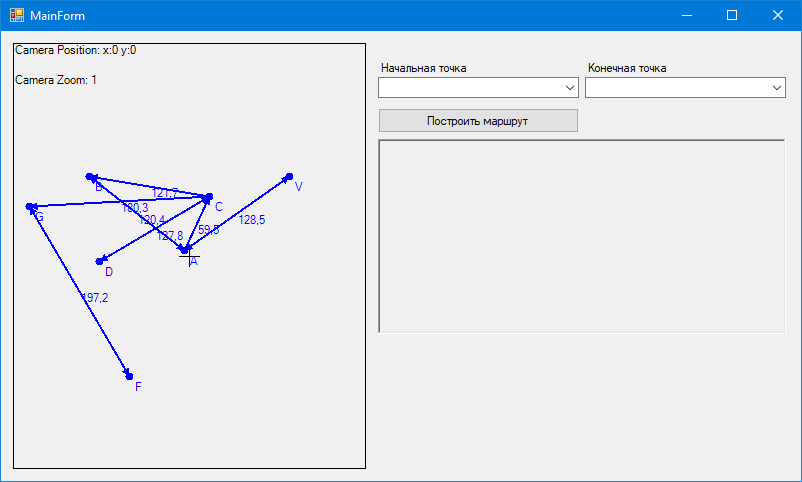
\includegraphics[width=1\textwidth]{menu}
Рисунок 1. Главное меню программы.
\end{center}

На рисунке 2 продемонстрирован выбор начального пункта A и конечного пункта B. Поскольку переместиться из пункта A в B возможно, маршрут был посмтроен в текстовое поле введено описания перемещения пройдённое расстояние из одной точки в другую, и общее расстояние.

\begin{center}
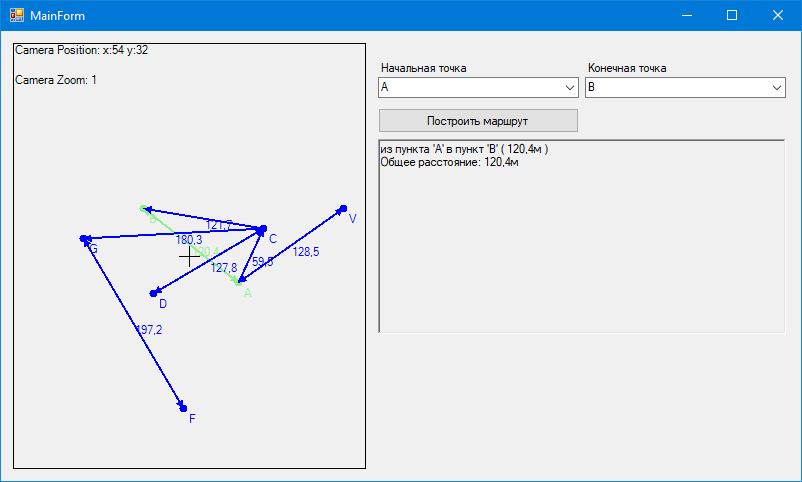
\includegraphics[width=1\textwidth]{atob}
Рисунок 2. Путь из точки A в точку B.
\end{center}

На рисунке 3 продемонстрирован выбор начального пункта A и конечного пункта A. Поскольку точки одинаковы, на компоненте отображения путей, ничего не было выделено, а в текстовом компоненте была описано пройденое расстояние, которое равна нулю.

\begin{center}
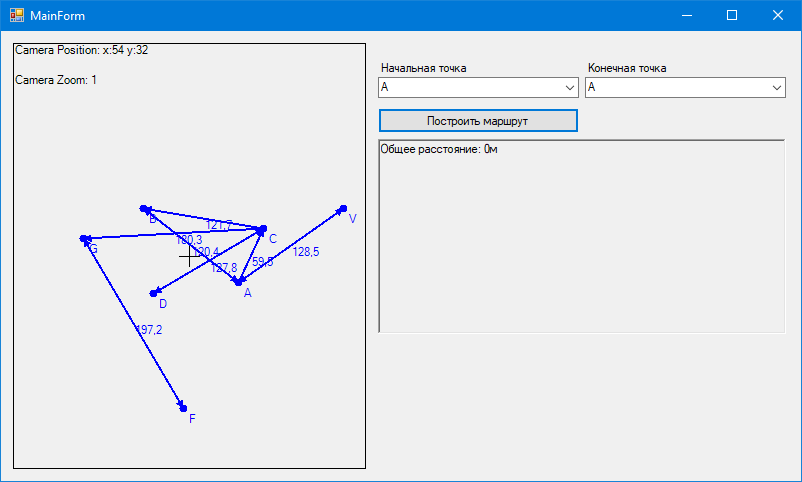
\includegraphics[width=1\textwidth]{atoa}
Рисунок 3. Путь из точки A в точку A.
\end{center}

На рисунке 4 продемонстрирован выбор начального пункта F и конечного пункта D. Переместиться из точки F в точку D невозможно, потому что по мере построения маршрута из точки G в точку C есть только односторонее движение из точки C в G, но не оборот, следовательно маршрут не был построен.

\begin{center}
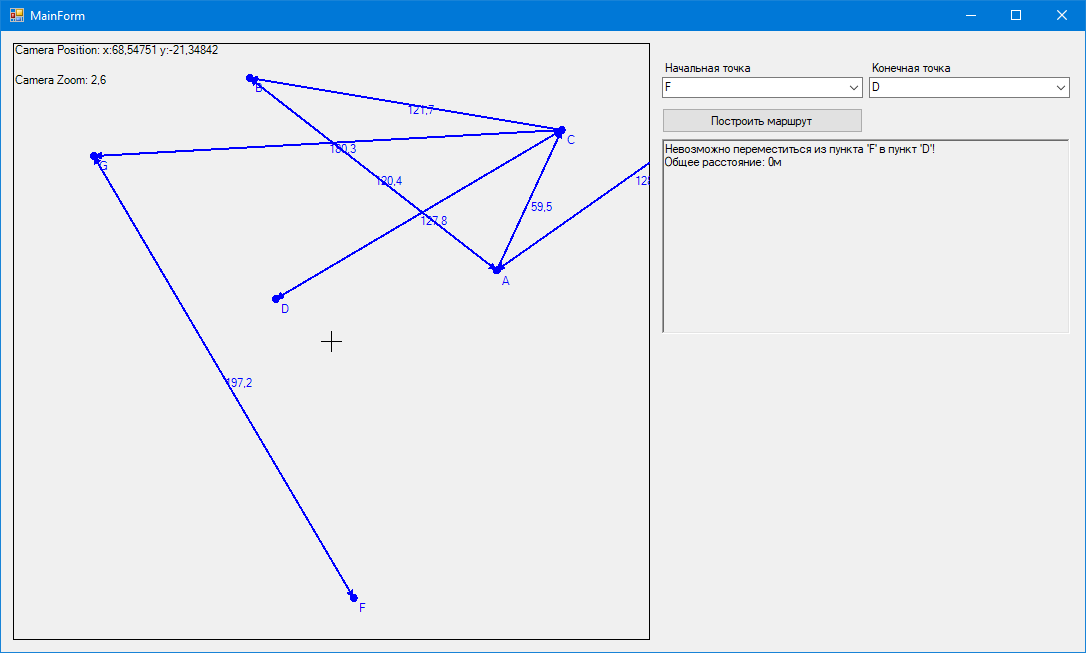
\includegraphics[width=1\textwidth]{atod}
Рисунок 4. Не удачный путь из точки F в точку D.
\end{center}


На рисунке 5 продемонстрирован выбор начального пункта V и конечного пункта F, на нём можно заметить как программа ставит множественные перемещения из одной точки в другую, и подбирает самый короткий путь, а именно V - A - C - G - F и в общем прошёл расстояние в 565,5м.

\begin{center}
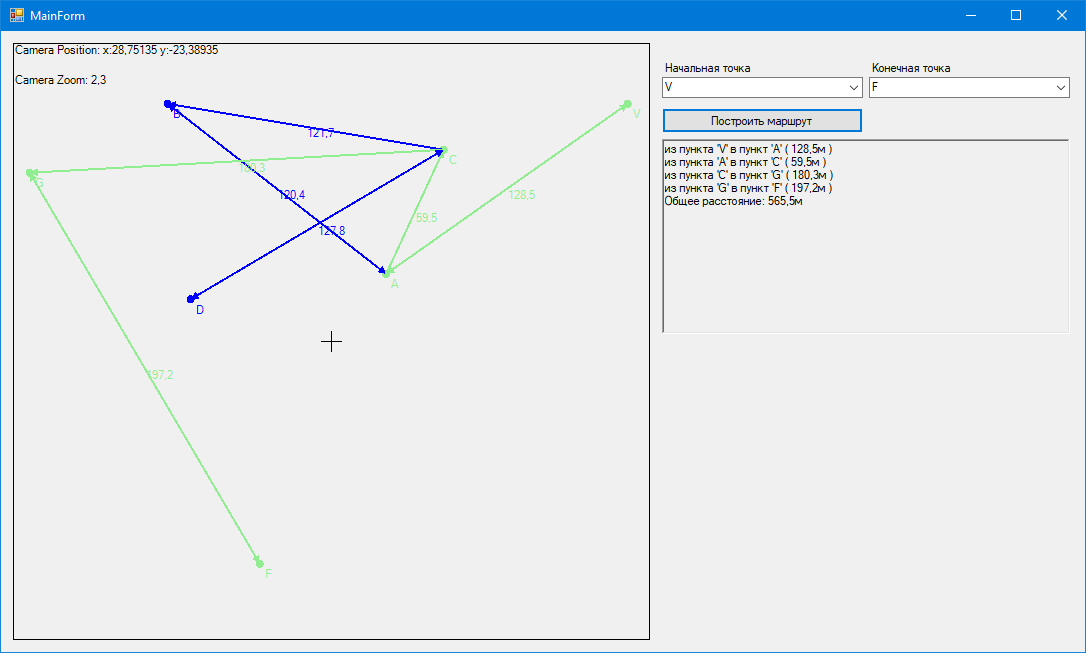
\includegraphics[width=1\textwidth]{vtof}
Рисунок 5. Путь из точки V в точку F.
\end{center}

\newpage
\section{ЗАКЛЮЧЕНИЕ}
В настоящее время происходит активное развитие информационных технологий. Повышение мощности компьютерной техники требует разработки нового программного обеспечения, способного выполнять разнообразные задачи по обработке информации. Появление нового поколения операционных систем требует разработку совместимых версий программного обеспечения. Специалисты предприятий всего мира уже не могут представить себе работу без вычислительной техники. Автоматизированное рабочее место повышает скорость и качество работы.

Программирование представляет собой вид высокоинтеллектуальной деятельности по разработке программного обеспечения. Составляется алгоритм будущей программы, который затем представляется в виде машинного текста, понятного для компьютера.

Для разработки программ используются различные языки программирования. Хороший программист должен уметь составлять алгоритмы решения и знать сразу несколько языков.

В заключение, можно сказать, что алгоритм Дейкстры является одним из наиболее эффективных методов нахождения кратчайшего пути в графах. Он позволяет быстро и точно находить кратчайшие пути между заданными вершинами, что делает его незаменимым инструментом в различных приложениях, таких как навигация, маршрутизация, планирование и т.д. Однако, как и любой другой алгоритм, он имеет свои ограничения и не всегда может быть применен в реальных задачах. Поэтому важно учитывать особенности конкретной задачи и выбирать оптимальный алгоритм для ее решения.

\newpage
\section{СПИСОК ИСТОЧНИКОВ}

\begin{enumerate}
  \item Простота использования: Windows Forms предоставляет интуитивно понятный интерфейс для создания пользовательского интерфейса приложения.
  \item Албахари, Дж. С\# 3.0. Справочник: Пер. с англ./ Дж. Албахари,  Б. Албахари. – 3-е изд. – Спб.: БХВ-Петербург, 2009. – 944 с.: ил.
  \item Окулов С.М. Программирование в алгоритмах. М.: Бином. Лаборатория знаний, 2004. 341 с.
  \item Юркин А.Г. Задачник по программированию. СПб.: Питер, 2002. 192 с.
  \item Ананий В. Левитин Глава 9. Жадные методы: Алгоритм Дейкстры // Алгоритмы: введение в разработку и анализ = Introduction to The Design and Analysis of Aigorithms. - М.: "Вильямс", 2006. - С.189-195.
  \item Томас Х. Кормен, Чарльз И. Лейзерсон, Рональд Л. Ривест, Клиффорд Штайн Алгоритмы: построение и анализ = Introduction to Algorithms. - 2-е изд. - М.: "Вильямс", 2006. - С.1296.
\end{enumerate}


\end{document}